\documentclass[10pt,aspectratio=169]{beamer}
%\usepackage{pgfpages}
% These slides also contain speaker notes. You can print just the slides,
% just the notes, or both, depending on the setting below. Comment out the want
% you want.

\setbeameroption{hide notes} % Only slides
%\setbeameroption{show only notes} % Only notes
%\setbeameroption{show notes on second screen=right} % Both

\usepackage{fsu2017}
% the aspect ratio defines the format
% default is 43 (4:3, 128mm:96mm), alternatives are
% 32 (3:2, 135mm:90mm)
% 54 (5:4, 125mm:100mm)
% 149 (14:9, 14cm:9cm)
% 169 (16:9, 16cm:9cm)
% 1610 (16:10, 16cm:10cm)
% 141 (1.41:1, 148.5mm:105mm, ratio of Din A)

\mode<presentation> {
\usetheme{Goettingen}
\setbeamertemplate{footline}[frame number] % To remove the footer line in all slides uncomment this line [page number] = for every page in PDF, [frame number] = for every frame
\setbeamerfont{footline}{size=\fontsize{8}{11}\selectfont}
%\setbeamerfont{section in sidebar}{size=\fontsize{7}{7}\selectfont}
%\setbeamerfont{subsection in sidebar}{size=\fontsize{7}{7}\selectfont}
%\setbeamerfont{subsubsection in sidebar}{size=\fontsize{7}{8}\selectfont}
%\setbeamertemplate{note page}[plain]

}
\makeatletter
\setbeamertemplate{sidebar canvas \beamer@sidebarside}%
                  [vertical shading][top=black!5!white,bottom=black!5!white]

\makeatother


\usepackage{color}
\usepackage{graphicx}
\usepackage{booktabs} % Allows the use of \toprule, \midrule and \bottomrule in tables
\usepackage{media9} % Allows videos
\usepackage{siunitx} % For Scientific SI units
\sisetup{output-exponent-marker=\ensuremath{\mathrm{e}}} % For 1e-10 being formatted nicely
\usepackage{hyperref}
\usepackage{pifont}% http://ctan.org/pkg/pifont
\newcommand{\cmark}{\ding{51}}%
\newcommand{\xmark}{\ding{55}}%
%\usepackage {tikz}
%\usepackage{tkz-graph}
%\usetikzlibrary {positioning}
%\usepackage {xcolor}
\AtBeginSection[]{
  \begin{frame}
  \vfill
  \centering
  \begin{beamercolorbox}[sep=8pt,center,shadow=true,rounded=true]{title}
    \usebeamerfont{title}\insertsectionhead\par%
  \end{beamercolorbox}
  \vfill
  \end{frame}
}
\setbeamercovered{invisible}
\setbeamercovered{%
  again covered={\opaqueness<1->{15}}}
%----------------------------------------------------------------------------------------
%	TITLE PAGE
%----------------------------------------------------------------------------------------

\title[Git, org-mode and mlflow for reproducibility]{Git, Emacs org-mode and mlflow: making applied machine learning research fully reproducible\\ \small{An extension of Stanisic et al, 2015}}
\author[Alex Seltmann\\Twitter \texttt{@aseltmann}\\\url{aseltmann.github.io}]{Alex Seltmann \inst{1,2}}
\institute{\inst{1} Institute of Applied Optic and Biophysics, Friedrich-Schiller University Jena, Max-Wien-Platz 1, 07743 Jena, Germany \and \inst{2} Leibniz-Institute of Photonic Technologies, Albert-Einstein Strasse 9, 07745 Jena, Germany}

\medskip
\date{\today}

\begin{document}

%% titlepage
\begin{frame}[noframenumbering]
	\titlepage
\end{frame}

%% TOC
%\begin{frame}
%    \frametitle{Overview} % Table of contents slide, comment this block out to remove it
%    \tableofcontents % \section{} and \subsection{} commands will automatically be printed
%\end{frame}

%----------------------------------------------------------------------------------------
%	PRESENTATION SLIDES
%----------------------------------------------------------------------------------------

\section{Scope}
\subsection{Computational research life cycle}
\begin{frame}{The computational research life cycle\footnote{Millman & Pérez (2018)}}
\tiny{
\begin{itemize}
  \item<1,5>
    \begin{Block}{Individual exploration}
        \only<1-4>{
        \begin{itemize}
            \item = single investiator tests idea, algorithm, question with
              small-scale dataset / simulation
            \item tools: Excel, Matlab, Mathematica, Sage, R, SPSS, ...
        \end{itemize}}
    \end{Block}
  \item<2,5>
    \begin{Block}{Collaboration}
        \only<2-4>{
        \begin{itemize}
            \item = bring together complementary expertise from colleagues
            \item tools: email, VCS, Dropbox, Github,
              (\texttt{paper-final-v2-REALLY-FINAL-john.doc})
        \end{itemize}}
    \end{Block}
  \item<3,5>
    \begin{Block}{Production-scale execution}
        \only<3-4>{
        \begin{itemize}
            \item = large data sets, complex simulations, supercomputers...
            \item tools: compiled code (C, C++, ...)
              and parallel computing libraries (MPI, Hadoop)
        \end{itemize}}
    \end{Block}
  \item<4,5>
    \begin{Block}{Publication \& Education}
        \only<4>{
        \begin{itemize}
            \item = paper, internal report, visualization $\to$ share with
              students and colleagues, cycle starts again
            \item tools: LATEX, Google Docs, Word, PowerPoint
        \end{itemize}}
    \end{Block}
\end{itemize}
}
  \only<5>{
    \begin{alertblock}{Goal: Use one setup for everything! Reduce manual data transfer!}
    \end{alertblock}
  }
  % Why??
  % 1. discontinuities between different stages of the scientific workflow - bc
  % of pressure to publish, people go always 'forward', assemble results  for
  % manucscript, but seldomly go back to update code, making reproducibility
  % hard
  % 2. manual transfer of info with manual changes after computational pipeline

% Note: problems are both technical and social - here focus on technical issues, but social reasons (publish or perish, no incentives, ...)
\end{frame}

\subsection{Definitions: reproducibility}
\begin{frame}{What are we talking about?\footnote{Goodman et al (2016)}}
    \begin{Block}{\textit{Methods} reproducibility}
        \begin{itemize}
            \item = get \textit{same} results, use \textit{same} data and tools
            \item topics: provide study protocols, reusable (meta)data, code,
              results, ...
        \end{itemize}
    \end{Block}
    \begin{alertblock}{Today: tools for methods reproducibility}
    \end{alertblock}
\end{frame}

\section{Tools}
\subsection{Org-mode}
\begin{frame}{What is org-mode}
    \begin{columns}[c]
    \begin{column}{.3\textwidth} % Left column and width
    \begin{minipage}{1\textwidth}
    \begin{itemize}
        \item<1>\textbf{plain text-based} tool for outlining, note-taking, spreadsheets, project planning, ...
        \item<2>\textbf{literate programming} via notebook-like environment for >70 programming languages
        \item<3>\textbf{one-click publishing} as HTML (or full-fledged modern website), LaTeX, ODT, ...
        \item<4>seemless git compatibility
    \end{itemize}
    % this together enables reproducible research via a consistent document consolidating the following 5 aspects which any reader can reproduce using the same tools
    % 1. exposition
    % 2. original data
    % 3. analyses
    % 4. discussion
    % 5. conclusion
    \end{minipage}
    \end{column}
    \begin{column}{.7\textwidth} % Right column and width
    \only<1>{
    \begin{figure}
        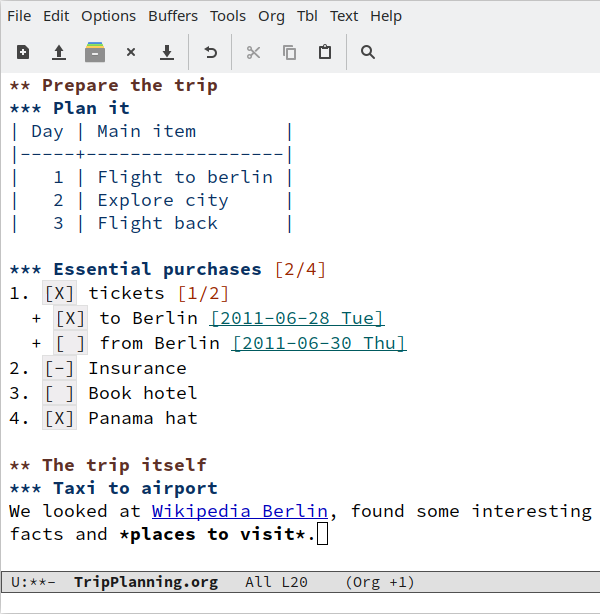
\includegraphics[height=0.8\textheight]{figures/tools_org-mode.png}
    \end{figure}}
    \only<2->{
    \begin{figure}
        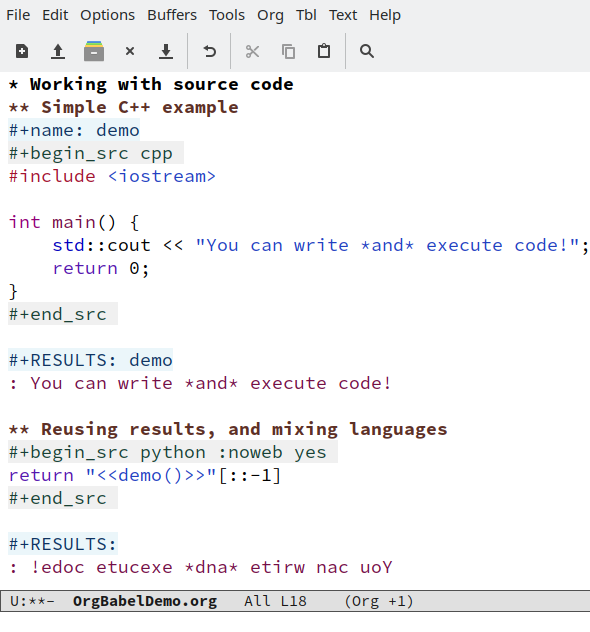
\includegraphics[height=0.8\textheight]{figures/tools_org-babel.png}
    \end{figure}}
    \end{column}\only<1>{\footnote{By Tecosaur - Own work, CC BY-SA 4.0, \tiny{\url{https://commons.wikimedia.org/w/index.php?curid=99366321}}}}
    \only<2->{\footnote{By Tecosaur - Own work, CC BY-SA 4.0,  \tiny{\url{https://commons.wikimedia.org/w/index.php?curid=99366428}}}}
    \end{columns}
\end{frame}

\subsection{Mlflow}
\begin{frame}{What is Mlflow}
    \begin{columns}[c]
    \begin{column}{.3\textwidth} % Left column and width
    \begin{minipage}{1\textwidth}
    \begin{itemize}
        \item<1>\textbf{Tracking}: API to log parameters, code, and results
        \item<2>\textbf{Projects}: code packaging format for reproducible runs using Conda and Docker
        \item<3>\textbf{Models}: model packaging format and tools for deployment (from any ML library)
    \end{itemize}
    \end{minipage}
    \end{column}
    \begin{column}{.7\textwidth} % Right column and width
    \only<1>{
    \begin{figure}
        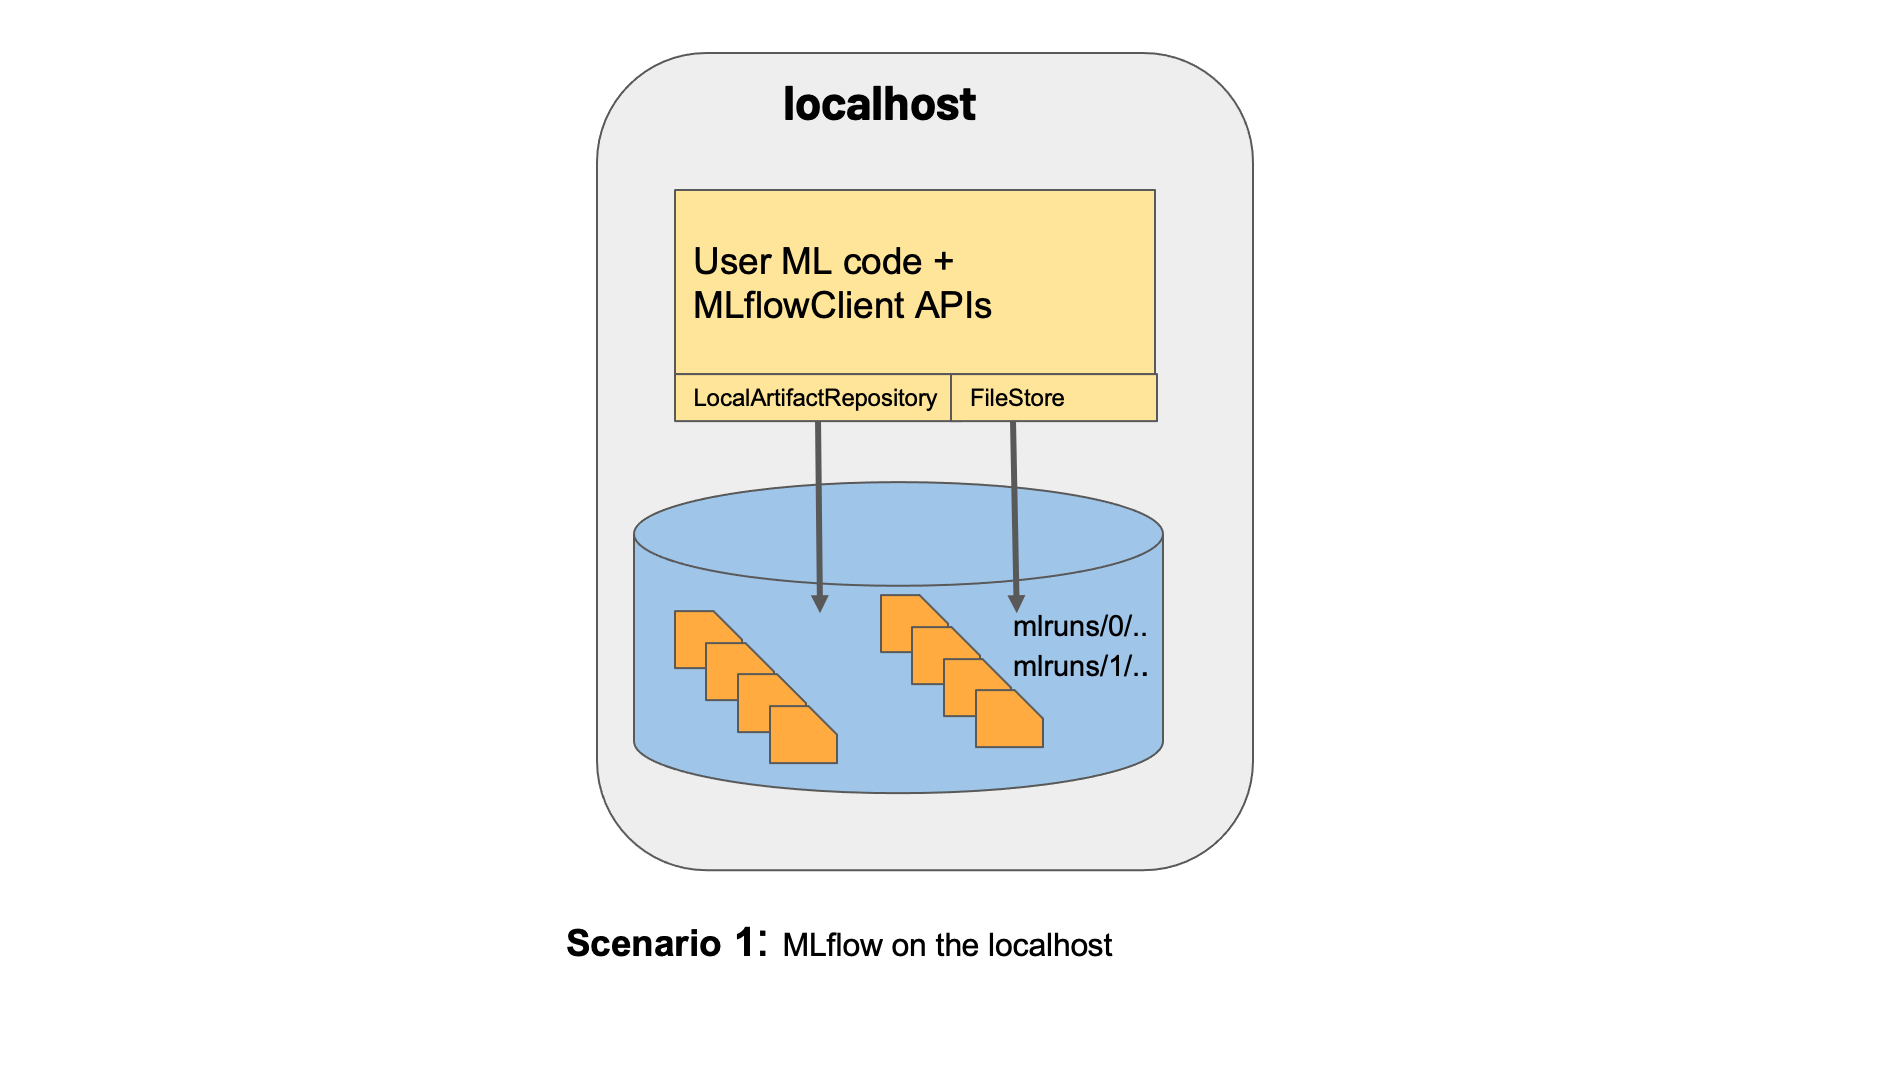
\includegraphics[height=0.75\textheight]{figures/tools_mlflow-tracking.png}
    \end{figure}}
    \only<2>{
    \begin{figure}
        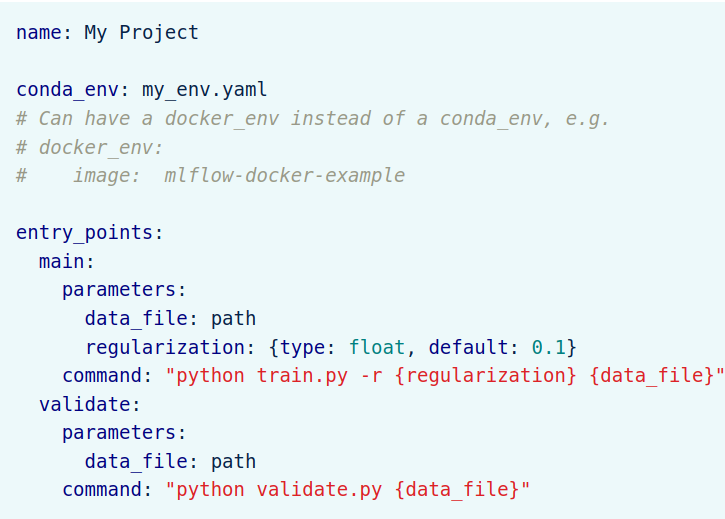
\includegraphics[height=0.75\textheight]{figures/tools_mlflow-projects.png}
    \end{figure}}
    \only<3>{
    \begin{figure}
        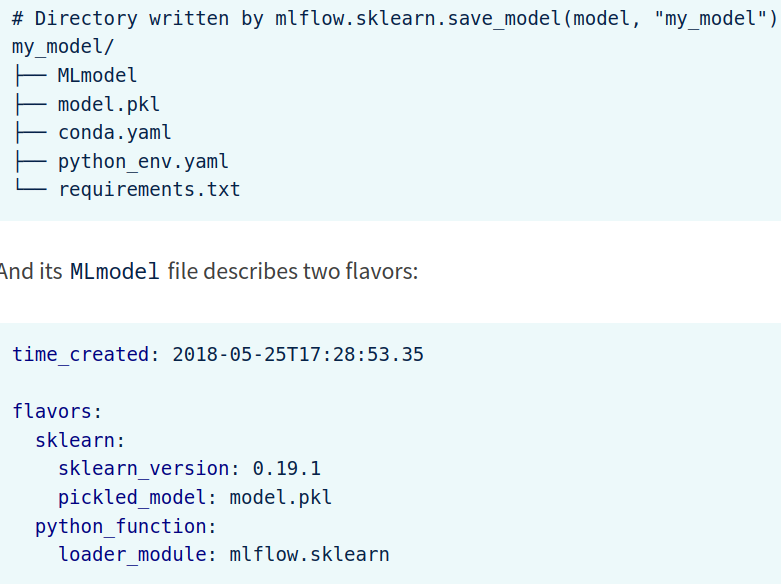
\includegraphics[height=0.75\textheight]{figures/tools_mlflow-models.png}
    \end{figure}}
    \end{column}\footnote{From MLflow documentation, CC BY 4.0, \tiny{\url{https://mlflow.org/docs/latest/projects.html}}}
    \end{columns}
\end{frame}

\subsection{Git}
\begin{frame}{Distributed Version Control with Git}
    \begin{figure}
        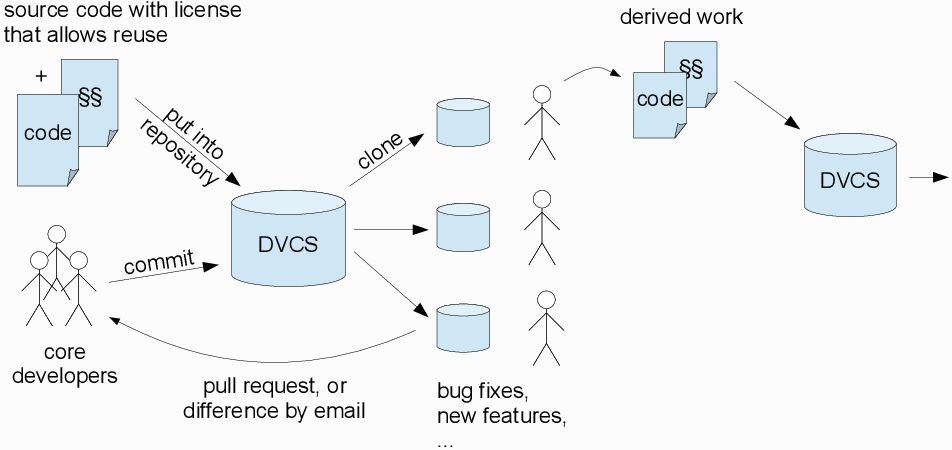
\includegraphics[width=\textwidth]{figures/tools_git.png}
    \end{figure}\footnote{Vanschoren, J., Braun, M.L., & Ong, C. (2018). Open science in machine learning. ArXiv, abs/1402.6013.}
\end{frame}

\section{Reproducible Workflow}
\begin{frame}{Motivation: bridge author-reader gap\footnote{Stanisic, L., Legrand, A., & Danjean, V. (2015). An Effective Git And Org-Mode Based Workflow For Reproducible Research. ACM SIGOPS Operating Systems Review, 49(1), 61–70. \tiny{\url{https://doi.org/10/gfbx5x}}
}}
    \begin{figure}
        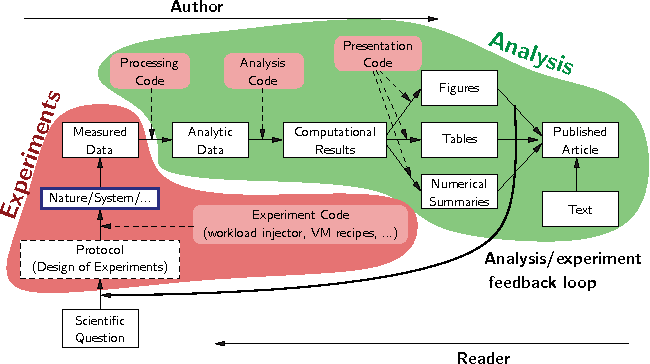
\includegraphics[width=0.9\textwidth]{figures/intro_motivation.png}
    \end{figure}
    
    % Bridging is achieved by
    % 1. opening the laboratory notebook (org-mode). All negative results and failures are shared as well
    % 2. version research process to facilitate reproduction
\end{frame}

\begin{frame}{Org-mode and Git for Reproducible Research\footnote{Stanisic, L., Legrand, A., & Danjean, V. (2015). An Effective Git And Org-Mode Based Workflow For Reproducible Research. ACM SIGOPS Operating Systems Review, 49(1), 61–70. \tiny{\url{https://doi.org/10/gfbx5x}}
}}
    \begin{columns}[c]
    \begin{column}{.3\textwidth} % Left column and width
    \begin{minipage}{1\textwidth}
    \begin{itemize}
        \item<1->\textbf{data file organization}: clear, coherent, hierarchical
        \item<2->\textbf{git branching structure}; version code, data, and results
        % \only<2>{\begin{itemize}
        %    \item track provenance, including failed experiments
        %    \item collaborate with others / keep project synced on multiple machines
        %    \item facilitate automated testing, code review, community feedback, ...
        %    \item clone individual experiments for reproduction
        % \end{itemize}}
        \item<3->\textbf{org-mode LabBook}: key analysis details
        % \only<3>{\begin{itemize}
        %    \item track provenance through literate programming
        %    \item links all scripts, programs, shell commands, parameters, data transformations
        %     \item flexible for individual exploration
        %    \item one-click executable for reproducing results
        % \end{itemize}}
    \end{itemize}
    % literate programming: 
    \end{minipage}
    \end{column}
    \begin{column}{.7\textwidth} % Right column and width
    \only<1>{
    \begin{figure}
        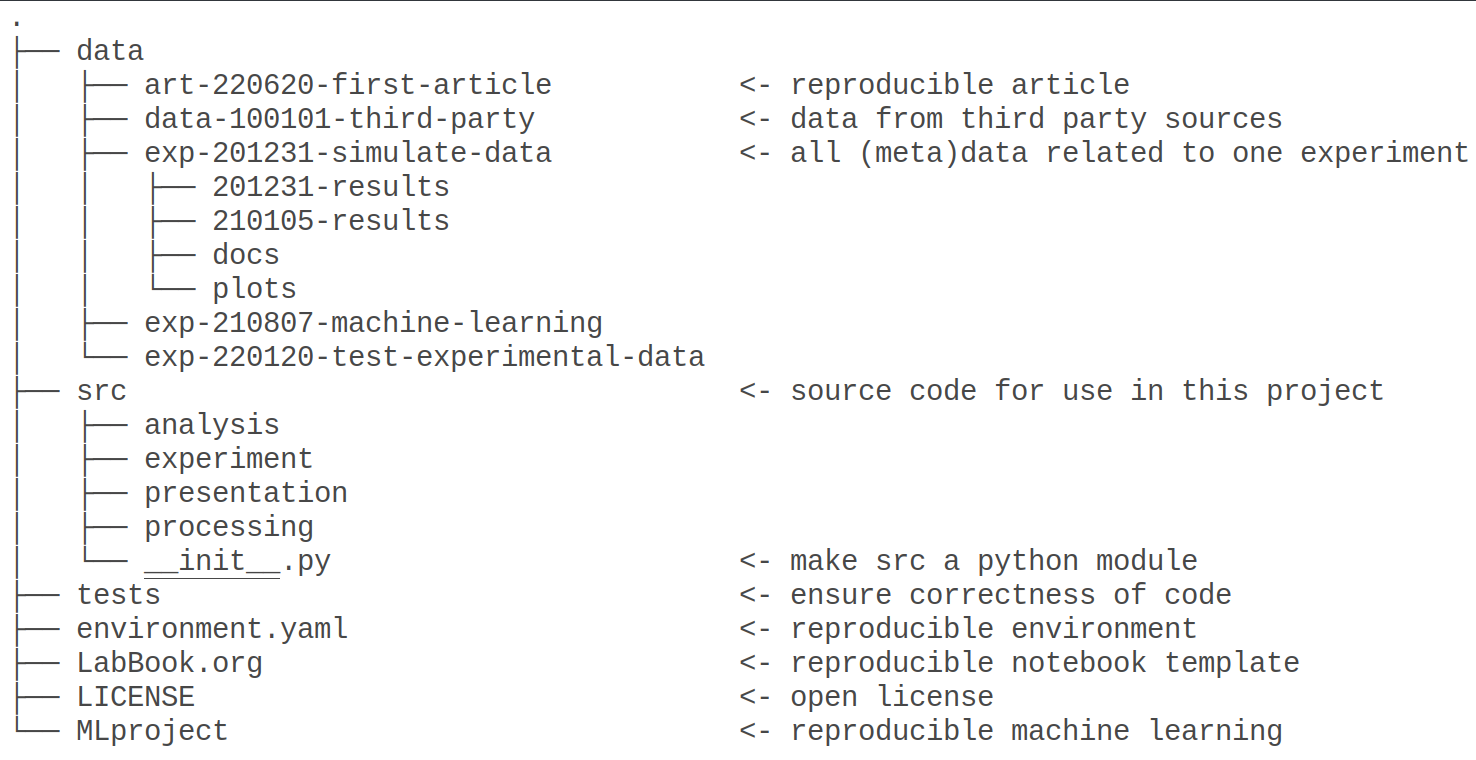
\includegraphics[width=\textwidth]{figures/workflow_structure.png}
    \end{figure}}
    \only<2>{
    \begin{figure}
        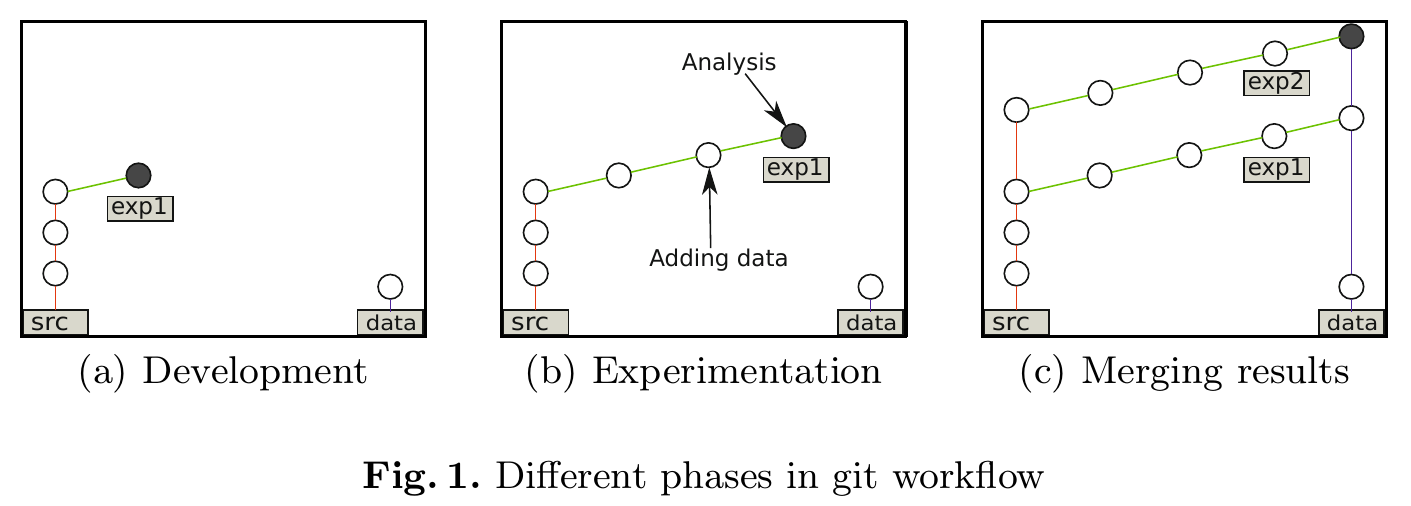
\includegraphics[width=\textwidth]{figures/workflow_phases.png}
    \end{figure}}
    \only<3>{
    \begin{figure}
        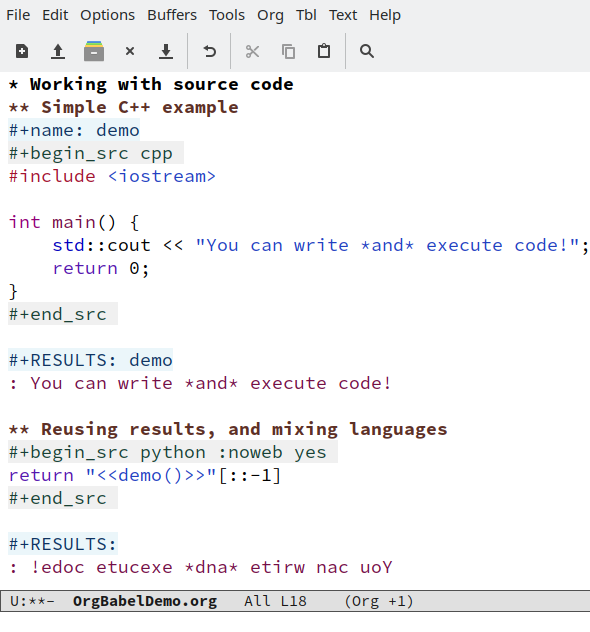
\includegraphics[height=0.75\textheight]{figures/tools_org-babel.png}
    \end{figure}}
    \end{column}
    \end{columns}
\end{frame}
\begin{frame}{Workflow Extension: mlflow + more}
    \begin{itemize}[<+->]
        \item \textbf{mlflow}: open source tool, that covers entire ML lifecycle and bridges the gap from ML research to application (e.g. model serving)
        \item \textbf{more practices adapted from open source development}: single-click dependency setup (e.g. Docker), automated unit testing (e.g. tox), automated code documentation (e.g. sphinx)
        \item \textbf{leveraging org-mode single-click publishing}: host website documenting every step of your experiments (\textit{Open Notebook Science}), easiest way to share experimental results including provenance
    \end{itemize}
\end{frame}

\section{Discussion}
\begin{frame}{Pros and Cons, Alternative Tools}
    \begin{columns}[c]
    \begin{column}{.5\textwidth} % Left column and width
    \begin{minipage}{1\textwidth}
    \begin{itemize}
        \item \textbf{Pros}
        \begin{itemize}
            \item combination of well-known, leightweight, open-source technologies
            \item facilitates reproducibility without taking away too much flexibility
        \end{itemize}
        \item \textbf{Cons}
        \begin{itemize}
            \item some conventions not commonly used (git branching model)
            \item steep learning curve (org-mode preferably with Emacs)
            \item large files (possible solutions: git lfs, git-annex)
        \end{itemize}
    \end{itemize}
    % literate programming: 
    \end{minipage}
    \end{column}
    \begin{column}{.5\textwidth} % Right column and width
    \visible<2>{
    \begin{itemize}
        \item \textbf{Alternatives}
        \begin{itemize}
            \item jupyter notebooks instead org-mode - more commonly used, more  intuitive, but not plain text (git integration), not the same flexbility
            \item R + knitr for literal programming
            \item 
        \end{itemize}
    \end{itemize}}
    \end{column}
    \end{columns}
\end{frame}

\begin{frame}{}
    \centering
    
\includegraphics[width=0.7\textwidth]{figures/meme_more-of-a-comment.jpg}
    \huge{\centerline{Questions?}}
\end{frame}
%------------------------------------------------

\begin{frame}{Acknowledgements}
    \begin{columns}[c]
    \column{.7\textwidth} % Left column and width
        \begin{figure}
            \centering
            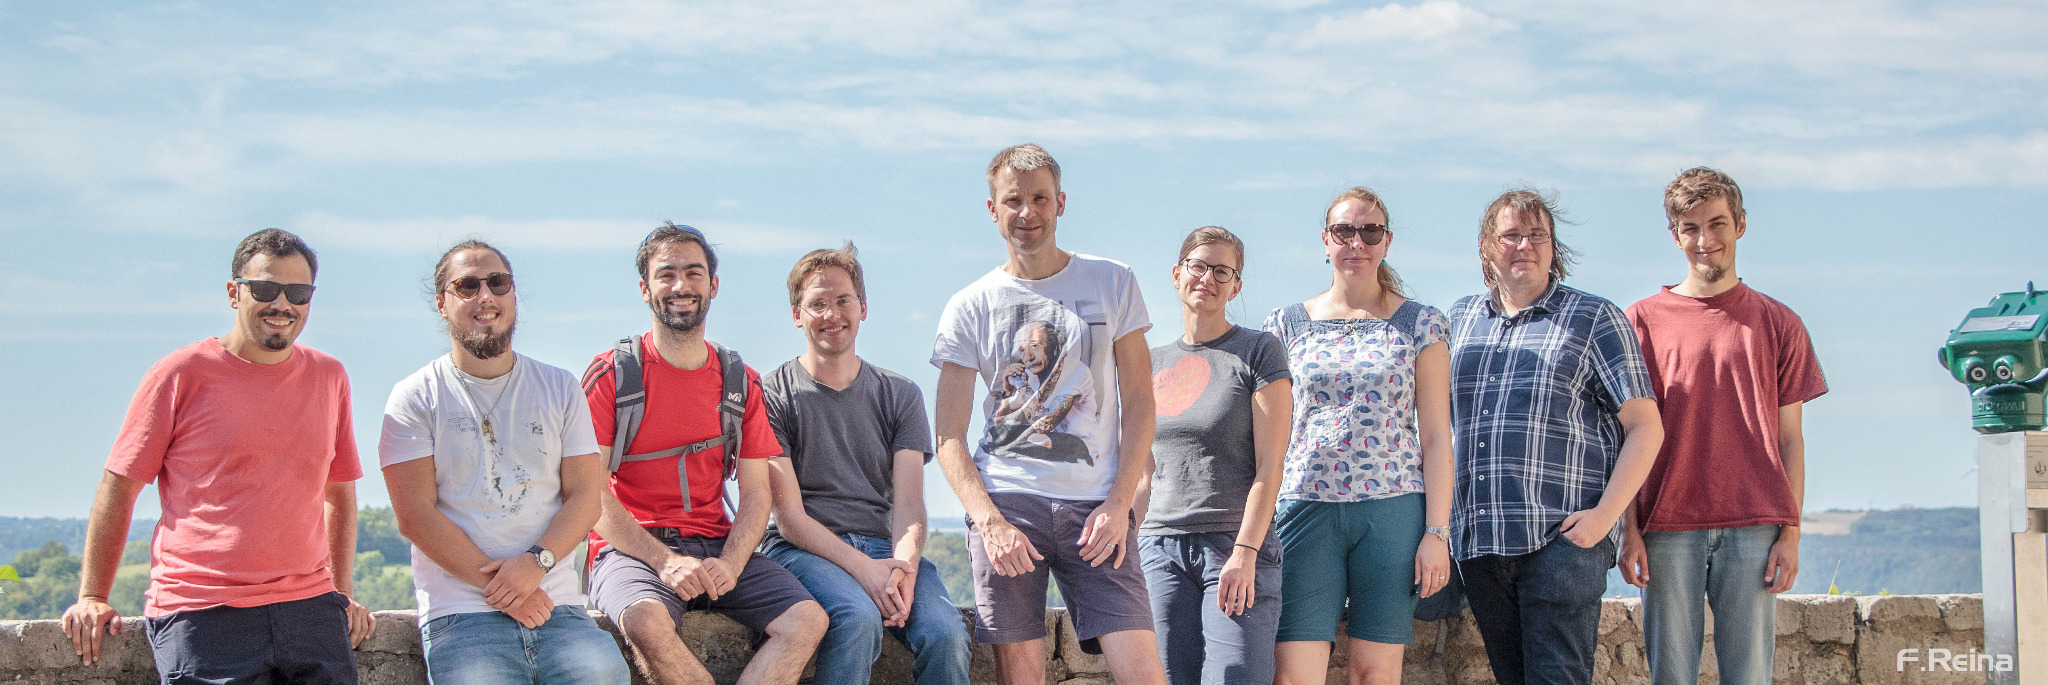
\includegraphics[width=1\textwidth]{figures/acknowledgements_groupfoto.jpeg}
        \end{figure}
        \begin{figure}
            \centering
            
\includegraphics[width=1\textwidth]{figures/acknowledgements_logos.jpeg}
        \end{figure}
        \par\noindent\rule{\textwidth}{0.4pt}
        \newline
        \begin{columns}[c]
        \column{.2\textwidth}
            \begin{figure}[c]
                \centering
                
\includegraphics[width=1\textwidth]{figures/by.pdf}
            \end{figure}
        \column{.75\textwidth}
            This work is licensed under a Creative Commons Attribution 4.0 International License.
        \end{columns}
    \column{.25\textwidth} % Right column and width
        \huge{\centerline{Thank you!}}
    \end{columns}
\end{frame}

\appendix
\newcounter{finalframe}
\setcounter{finalframe}{\value{framenumber}}

% Backup frames
\begin{frame}{Extra: Resources}
    \begin{columns}[c]
    \begin{column}{.3\textwidth} % Left column and width
    \begin{minipage}{1\textwidth}
    \begin{itemize}
        \item from comment after talk: DataLad as alternative to git
        \item Open online course to learn git and org-mode
    \end{itemize}
    \end{minipage}
    \end{column}
    \begin{column}{.7\textwidth} % Right column and width
    \begin{figure}
        
\includegraphics[width=\textwidth]{figures/extra_course.png}
     \end{figure}
    \end{column}
    \end{columns}\footnote{\url{http://handbook.datalad.org/en/latest/index.html#}}\footnote{\url{https://www.fun-mooc.fr/en/courses/reproducible-research-methodological-principles-transparent-scie/}}
\end{frame}

\begin{frame}{Extra: Mlflow UI}
    \begin{figure}
        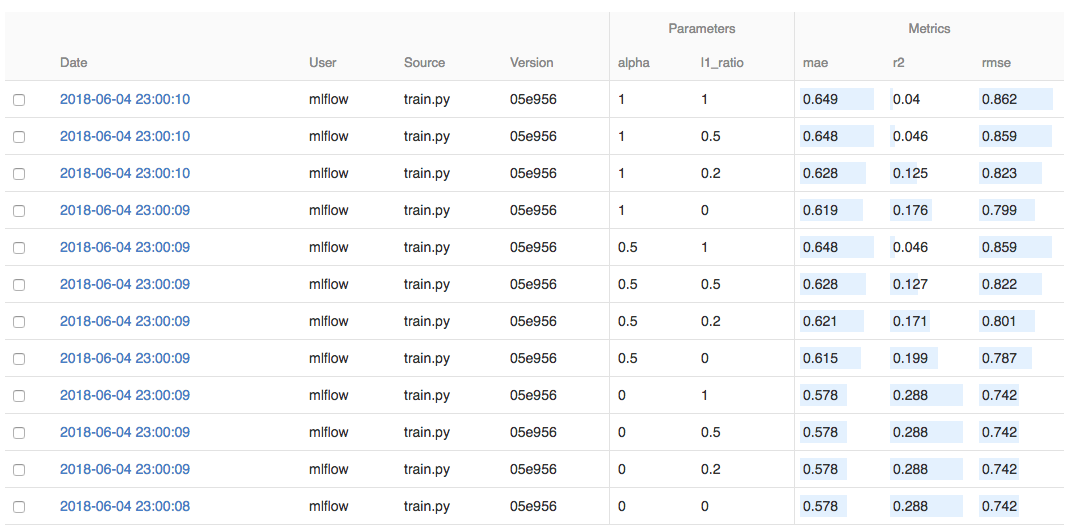
\includegraphics[width=\textwidth]{figures/tools_mlflow-ui.png}
    \end{figure}\footnote{From MLflow documentation, CC BY 4.0, \tiny{\url{https://mlflow.org/docs/latest/projects.html}}}
\end{frame}

\begin{frame}{Extra: fields of Open Science covered}
    \begin{figure}
        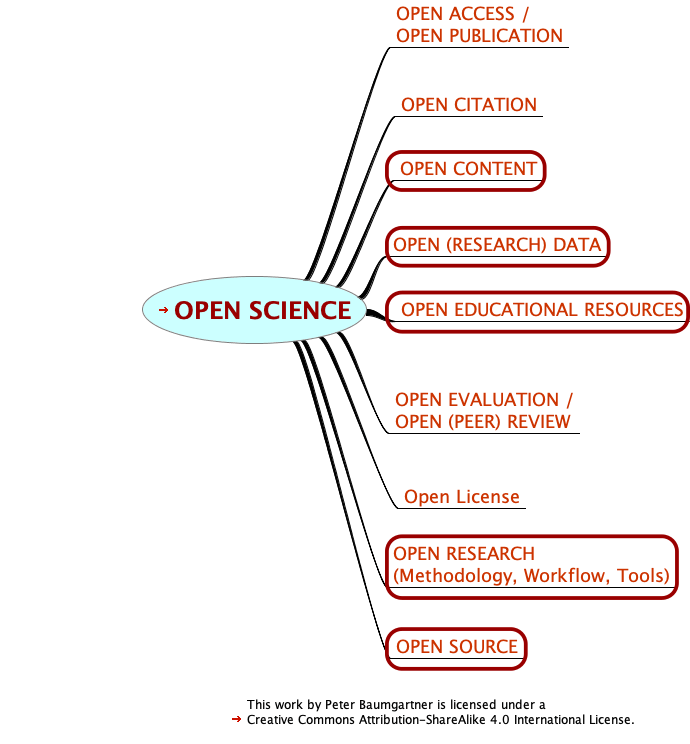
\includegraphics[height=0.9\textheight]{figures/intro_open-science-baumgartner_marked.png}
    \end{figure}
\end{frame}

\begin{frame}{Extra: other definitions of reproducibility\footnote{Goodman et al (2016)}}
\small{
    \begin{Block}{\textit{Methods} reproducibility}
        \begin{itemize}
            \item = get \textit{same} results, use \textit{same} data and tools
            \item topics: provide study protocols, reusable (meta)data, code,
              results, ...
        \end{itemize}
    \end{Block}
    \begin{Block}{\textit{Results} reproducibility = replication}
        \begin{itemize}
            \item = get \textit{similar} results, use \textit{similar}
              procedures and tools (maybe different data)
            \item topics: statistical significance, cumulative evidential
              weight, heterogeneity tests, effect sizes...
        \end{itemize}
    \end{Block}
    \begin{Block}{\textit{Inferential} reproducibility}
        \begin{itemize}
            \item = get same scientific conclusions from independent study or
              re-analysis of the data, use \textit{different} tools and methods
            \item topics: bayesian perspectives, avoiding multiplicity, HARKing,
              p-hacking
        \end{itemize}
    \end{Block}
}
\end{frame}

\setcounter{framenumber}{\value{finalframe}}
%----------------------------------------------------------------------------------------
\end{document}
%------------------------------------------------------ 